\section{Results}
\label{sec:results}

\subsection{Headline three-way comparison}
Table~\ref{tab:threeway} and Figure~\ref{fig:fig1} summarize every grader on
both labeled testbeds under a single metric definition
(\S\ref{sec:protocol}): \emph{strict} recall (abstain-on-error counts as a miss)
and FPR among covered negatives. The pattern is consistent. The symbolic
verifier commits on only $47.1\%$ of human-labeled steps and $35.6\%$ of
injection trials; where it commits it is essentially never wrong (injection
precision $1.00$, FPR $0.00$), but its strict recall is $0.000$ on the 13 human
errors and only $0.234$ on injected errors. Both LLM judges instead commit
almost everywhere (coverage $\geq 0.92$) and agree with far more of the human
error labels (strict recall $0.462$ for \texttt{gpt-oss} and $0.769$ for
\texttt{claude}; injection recall $0.851$ and $0.904$), but they pay for it in
false positives, with injection FPR $0.087$ and $0.182$ respectively, while the
symbolic verifier's FPR stays at $0$. These injection FPR values rest on few
covered negatives (20, 23, and 22 covered non-errors out of 24 total, for
symbolic, \texttt{gpt-oss}, and \texttt{claude}); the
\texttt{gpt-oss}--\texttt{claude} gap is 2 vs.\ 4 false positives, and $95\%$
Wilson intervals are wide and overlapping ($[0.024, 0.268]$ vs.\ $[0.073,
0.385]$), so the FPR ordering is directional rather than precisely estimated.
Human-set precision/recall are agreement
with a rubric the judges did not see (\S\ref{sec:protocol}).

\begin{table*}[t]
\centering
\footnotesize
\setlength{\tabcolsep}{2.8pt}
\begin{tabular}{llrrrrrrrrrr}
\toprule
dataset & grader & cov. & prec. & rec. & FPR & abst. & TP & FP & TN & FN & AbsE \\
\midrule
\multirow{3}{*}{human}
 & symbolic & 0.471 & n/a & 0.000 & 0.000 & 0.529 & 0 & 0 & 83 & 7 & 6 \\
 & \texttt{gpt-oss-120b} & 0.995 & 0.667 & 0.462 & 0.017 & 0.005 & 6 & 3 & 175 & 6 & 1 \\
 & \texttt{claude-sonnet-4-5} & 0.953 & 0.370 & 0.769 & 0.100 & 0.047 & 10 & 17 & 153 & 2 & 1 \\
\midrule
\multirow{3}{*}{injection}
 & symbolic & 0.356 & 1.000 & 0.234 & 0.000 & 0.644 & 22 & 0 & 20 & 0 & 72 \\
 & \texttt{gpt-oss-120b} & 0.941 & 0.976 & 0.851 & 0.087 & 0.059 & 80 & 2 & 21 & 8 & 6 \\
 & \texttt{claude-sonnet-4-5} & 0.924 & 0.955 & 0.904 & 0.182 & 0.076 & 85 & 4 & 18 & 2 & 7 \\
\bottomrule
\end{tabular}
\caption{Three-way grader comparison on the human-labeled ($n{=}191$ steps; 13
errors) and error-injection ($n{=}118$ applicable trials; 94 errors, 24
non-errors) testbeds. \textbf{One definition throughout:} coverage $=$ committed
fraction; precision $=\mathrm{TP}/(\mathrm{TP}+\mathrm{FP})$; \emph{strict}
recall $=\mathrm{TP}/(\mathrm{TP}+\mathrm{FN}+\mathrm{AbsE})$ (abstain-on-error
is a miss); FPR $=\mathrm{FP}/(\mathrm{FP}+\mathrm{TN})$ on covered negatives.
TP/FP/TN/FN are among committed verdicts only; AbsE $=$ abstain or
unparseable/crash on a true-error case. Identity:
$\mathrm{TP}+\mathrm{FP}+\mathrm{TN}+\mathrm{FN}+\mathrm{AbsE}+\mathrm{AbsN}=n$
(AbsN omitted for space; see \texttt{threeway\_table.json}). On the human set,
precision/recall measure agreement with the human rubric the LLM judges were
not shown (\S\ref{sec:protocol}). Human-set recall denominators are all 13
errors, matching Table~\ref{tab:paired}.}
\label{tab:threeway}
\end{table*}

\begin{figure}[t]
\centering
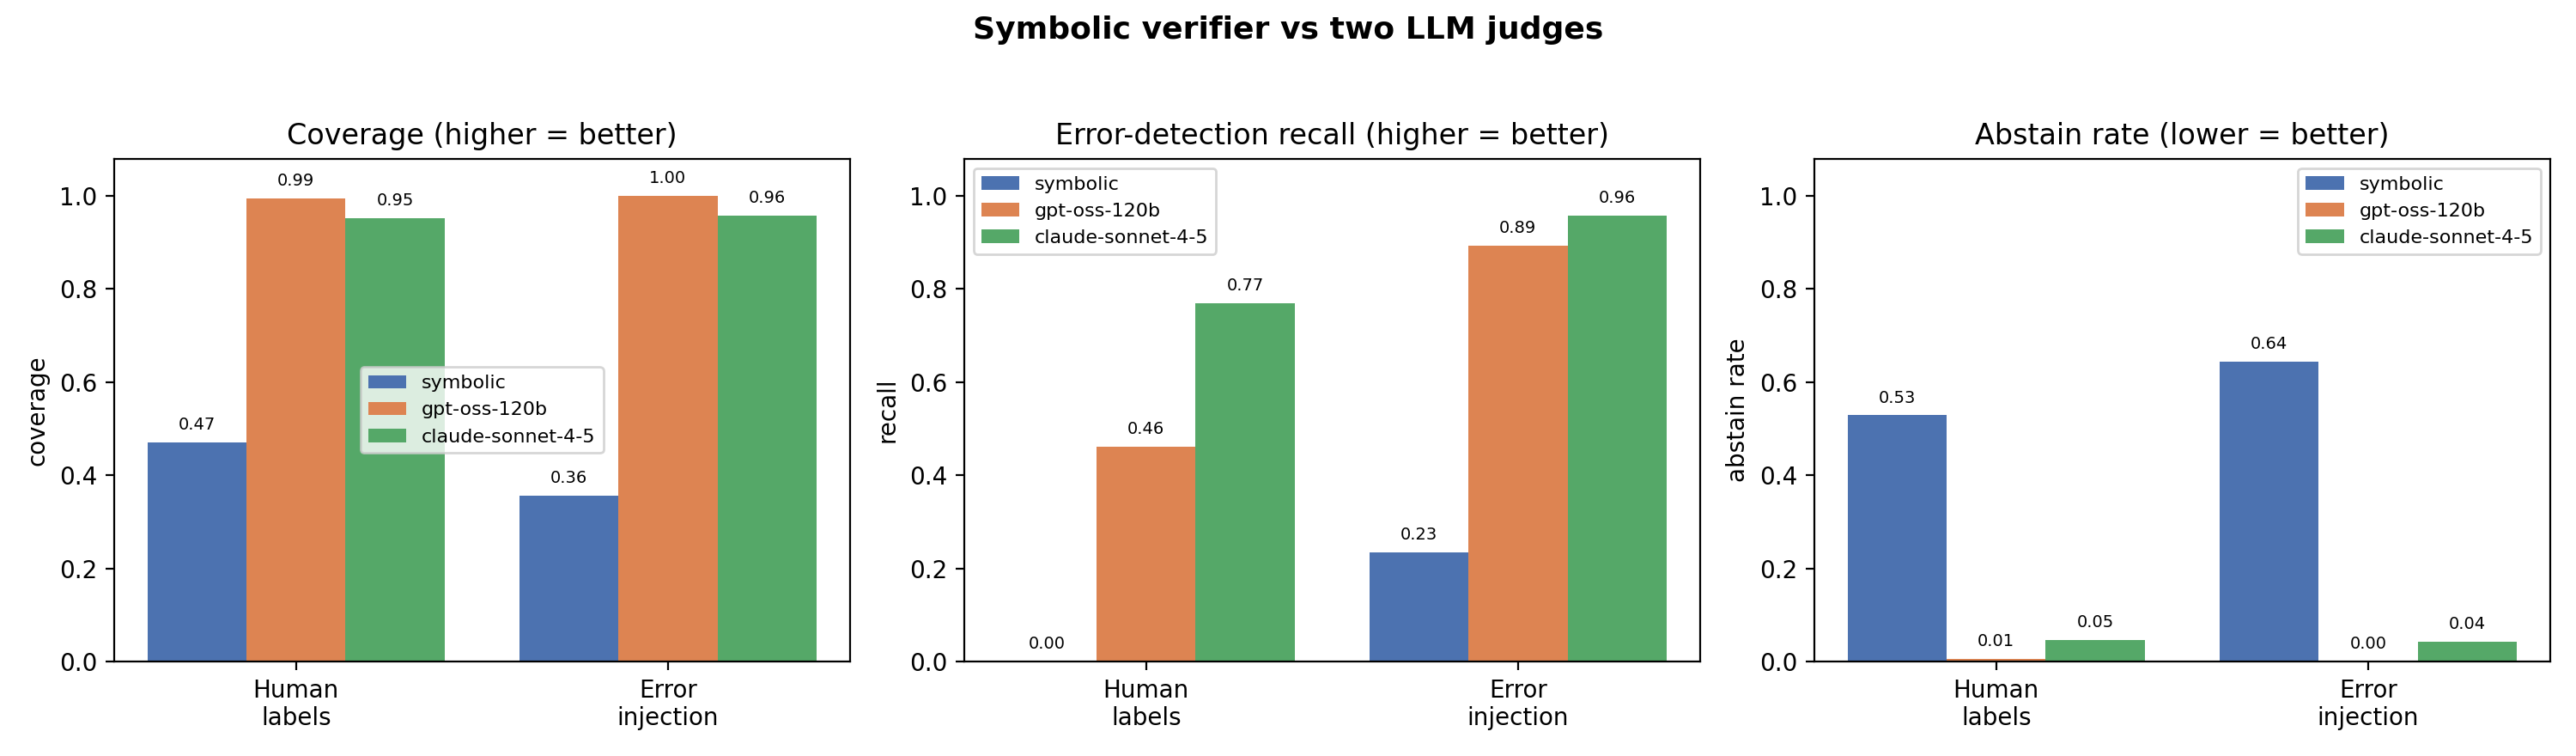
\includegraphics[width=\columnwidth]{../results/figures/fig1_grader_comparison.png}
\caption{Coverage, strict error-detection recall, and abstention for the three
graders on both testbeds. Symbolic trades coverage for zero false positives; the
LLM judges do the opposite.}
\label{fig:fig1}
\end{figure}

\subsection{Paired significance on the human set}
Table~\ref{tab:paired} reports the paired step-level comparison of each judge
against the symbolic verifier on the same 191 steps. Exact McNemar tests with
Holm--Bonferroni correction over the six-test family
\citep{dror2018hitchhikers} reject the null for all six comparisons at
$\alpha{=}0.05$: both judges have higher coverage and
correct\_committed rates than symbolic ($p_{\mathrm{Holm}}\!\ll\!0.001$), and
higher strict recall on the 13 error steps
($p_{\mathrm{Holm}}{=}0.031$ for \texttt{gpt-oss}, $0.0039$ for
\texttt{claude}). Point estimates match Table~\ref{tab:threeway}
($\Delta_{\mathrm{caught}}{=}{+}0.46$ and ${+}0.77$). Bootstrap CIs for
\texttt{caught\_error} are omitted as uninformative ($n{=}13$; Claude's would
reach the boundary $1$; Limitations).

\begin{table}[t]
\centering
\small
\resizebox{\columnwidth}{!}{%
\begin{tabular}{llrll}
\toprule
judge & metric & $\Delta$ & 95\% CI & McNemar $p$ / Holm $p$ \\
\midrule
\multirow{3}{*}{\texttt{gpt-oss}}
 & committed          & $+0.524$ & $[0.450, 0.592]$ & $<\!10^{-20}$ / $<\!10^{-20}$ \\
 & correct\_committed & $+0.513$ & $[0.440, 0.586]$ & $<\!10^{-20}$ / $<\!10^{-20}$ \\
 & caught\_error      & $+0.46$ & uninf.\ ($n{=}13$) & $0.031$ / $0.031$ \\
\midrule
\multirow{3}{*}{\texttt{claude}}
 & committed          & $+0.482$ & $[0.403, 0.560]$ & $<\!10^{-20}$ / $<\!10^{-20}$ \\
 & correct\_committed & $+0.419$ & $[0.335, 0.497]$ & $<\!10^{-17}$ / $<\!10^{-16}$ \\
 & caught\_error      & $+0.77$ & uninf.\ ($n{=}13$; hits 1) & $0.0020$ / $0.0039$ \\
\bottomrule
\end{tabular}%
}
\caption{Paired step-level differences (judge $-$ symbolic). Primary test:
exact McNemar on discordant pairs; Holm--Bonferroni over six tests
($\alpha{=}0.05$). Bootstrap CIs are descriptive where shown; omitted for
\texttt{caught\_error} ($n{=}13$; uninformative, since Claude's interval would
reach 1).}
\label{tab:paired}
\end{table}

\subsection{Cascade: symbolic first, judge on abstain}
\label{sec:cascade}

Run the symbolic verifier first and invoke an LLM judge only when it abstains.
We evaluate that cascade
\emph{post hoc} on the frozen verdicts (no new model calls) against all three
standalone graders (Table~\ref{tab:cascade}). The rule is fixed: if symbolic
commits, take its verdict; else take the judge; else abstain. Metrics match
Table~\ref{tab:threeway}.

\begin{table*}[t]
\centering
\footnotesize
\setlength{\tabcolsep}{2.5pt}
\begin{tabular}{llrrrrrr}
\toprule
dataset & grader & cov. & prec. & rec. & FPR & abst. & (sym / judge / abs) \\
\midrule
\multirow{5}{*}{human}
 & symbolic & 0.471 & n/a & 0.000 & 0.000 & 0.529 & --- \\
 & \texttt{gpt-oss} & 0.995 & 0.667 & 0.462 & 0.017 & 0.005 & --- \\
 & \texttt{claude} & 0.953 & 0.370 & 0.769 & 0.100 & 0.047 & --- \\
 & cascade$\rightarrow$\texttt{gpt-oss} & 0.995 & 0.600 & 0.231 & 0.011 & 0.005 & 90 / 100 / 1 \\
 & cascade$\rightarrow$\texttt{claude} & 0.984 & 0.263 & 0.385 & 0.080 & 0.016 & 90 / 98 / 3 \\
\midrule
\multirow{5}{*}{injection}
 & symbolic & 0.356 & 1.000 & 0.234 & 0.000 & 0.644 & --- \\
 & \texttt{gpt-oss} & 0.941 & 0.976 & 0.851 & 0.087 & 0.059 & --- \\
 & \texttt{claude} & 0.924 & 0.955 & 0.904 & 0.182 & 0.076 & --- \\
 & cascade$\rightarrow$\texttt{gpt-oss} & 0.966 & 0.976 & 0.872 & 0.083 & 0.034 & 42 / 72 / 4 \\
 & cascade$\rightarrow$\texttt{claude} & 0.941 & 0.988 & \textbf{0.904} & \textbf{0.042} & 0.059 & 42 / 69 / 7 \\
\bottomrule
\end{tabular}
\caption{Standalone graders vs.\ the symbolic$\rightarrow$LLM cascade (same
metric definitions as Table~\ref{tab:threeway}). Rightmost column: how many
cascade decisions came from symbolic, from the judge, or remained abstain.
On injection, cascade$\rightarrow$\texttt{claude} keeps Claude's recall while
cutting FPR from $0.182$ to $0.042$; cascade$\rightarrow$\texttt{gpt-oss} raises
recall over the judge alone ($0.851\rightarrow 0.872$) at matched precision. On
the human set both cascades \emph{lose} recall relative to the judge alone,
because the verifier's 7 committed passes on human-error steps (5
mid-derivation false passes, 2 first-step definitional passes;
Table~\ref{tab:human-errors}) are locked in and never reach the judge.}
\label{tab:cascade}
\end{table*}

On the injection suite the cascade is a clear win. Symbolic contributes its
high-precision commits (42/118 trials); the judge covers most abstains. With
\texttt{claude} as the fallback, recall stays at $0.904$ while FPR drops from
$0.182$ to $0.042$ and precision rises to $0.988$, the best injection operating
point in the study. With \texttt{gpt-oss}, recall improves on the judge alone
($0.851\rightarrow 0.872$) at essentially unchanged precision/FPR.

On the human set the same policy backfires on recall. Symbolic commits on
90/191 steps, including all 7 committed passes on human-error steps (5
mid-derivation false passes plus 2 first-step definitional passes;
Table~\ref{tab:human-errors}; Table~\ref{tab:threeway}, FN$=7$). The cascade
trusts those passes, so the judge never sees them:
cascade$\rightarrow$\texttt{gpt-oss} recall falls from $0.462$ to $0.231$, and
cascade$\rightarrow$\texttt{claude} from $0.769$ to $0.385$. Coverage stays high
and FPR edges down, but the errors the verifier is blind to become irreversible
false negatives. This degradation is deterministic given the verifier's
false-pass count, a structural warning about cascade design rather than a
corpus-specific result. The prescription is therefore conditional: \textbf{cascade when
symbolic commits are trustworthy} (algebraic / injection-like regimes);
\textbf{do not let symbolic passes veto the judge} on steps outside the symbolic
fragment (\S\ref{sec:analysis}).

\paragraph{Cost and latency price tag.}
``Use both'' needs a bill. Symbolic verification is local CPU at effectively
$\$0$ ($\approx\!60$\,ms/step, $\approx 11$\,s total on the 191 human steps on
one laptop CPU; absolute timings are machine-dependent), and because it
already commits on the steps it can verify, the cascade cuts LLM calls by
$47\%$ on the human set ($191\!\rightarrow\!101$) and $36\%$ on injection
($118\!\rightarrow\!76$). Estimated dollar costs at published list rates fall
by the same fraction (Appendix~\ref{app:cost}), but rate cards change; the
call-count reduction does not, and any deployment can measure it directly
without our prices.

\subsection{Confidence thresholding: precision--coverage curves}
\label{sec:confidence}

Each LLM judge already returns a confidence in $[0,1]$ with every verdict
(Appendix~\ref{app:prompt}); prior sections ignored it. We recover a family of
operating points \emph{for free} by committing only when
$\mathrm{confidence}\ge\tau$ and abstaining otherwise
(Figure~\ref{fig:fig3}). Coverage is a dial, not a fixed property of the model.

On the human set, raising $\tau$ trades recall for precision. \texttt{gpt-oss}
at $\tau{=}0.95$ moves precision $0.667\!\rightarrow\!0.833$ and FPR
$0.017\!\rightarrow\!0.006$ at coverage $0.927$, but recall falls
$0.462\!\rightarrow\!0.385$. \texttt{claude} at $\tau{=}0.90$ moves precision
$0.370\!\rightarrow\!0.500$ and FPR $0.100\!\rightarrow\!0.026$ at coverage
$0.848$, at a steeper recall cost ($0.769\!\rightarrow\!0.308$) since its
catches concentrate in lower-confidence verdicts. Thresholding is a
false-positive control, not a free improvement, and these are illustrative
in-sample operating points; a deployment would calibrate $\tau$ on held-out
data. On injection, high $\tau$ pushes \texttt{gpt-oss} toward precision $1.0$
(coverage $0.466$ at $\tau{=}0.99$), while \texttt{claude}'s more compressed
confidences give a flatter curve; both move along the same precision/recall
frontier rather than escaping it (complementary to the cascade of
\S\ref{sec:cascade}).

\begin{figure}[t]
\centering
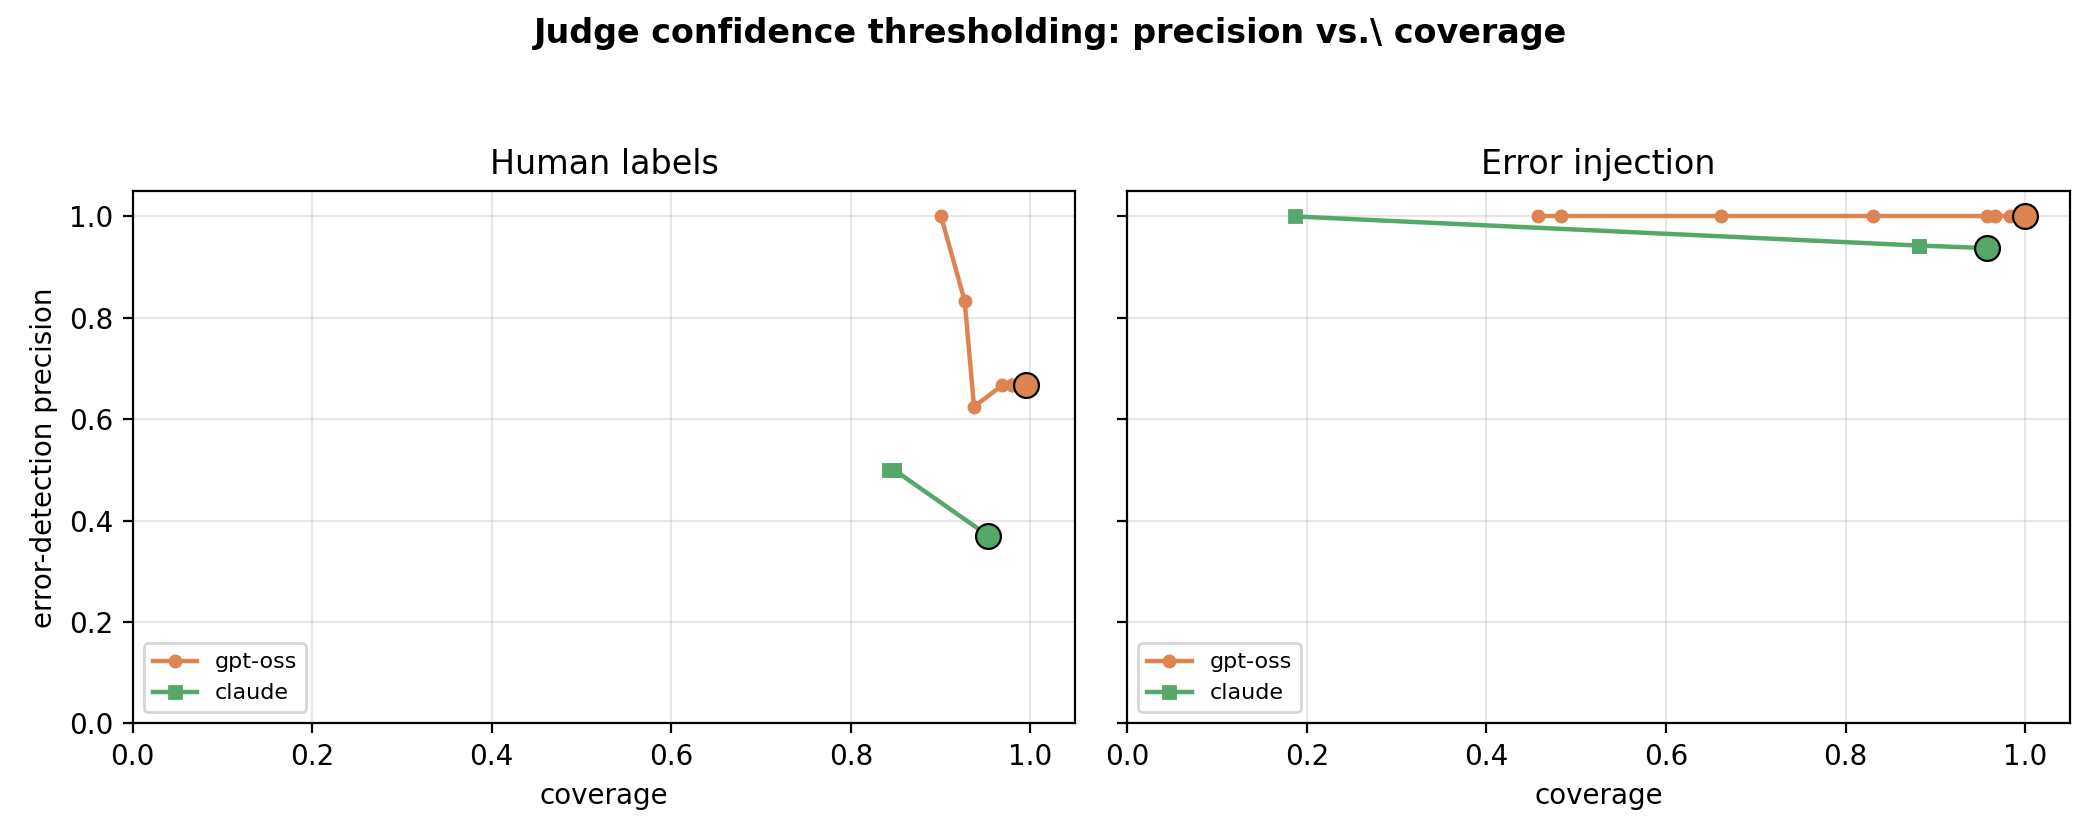
\includegraphics[width=\columnwidth]{../results/figures/fig3_precision_coverage.png}
\caption{Error-detection precision vs.\ coverage under confidence thresholding
(commit iff $\mathrm{confidence}\ge\tau$). Black-edged markers are the default
operating points ($\tau{=}0$) from Table~\ref{tab:threeway}. Curves use only
frozen judge outputs; no new API calls.}
\label{fig:fig3}
\end{figure}

\subsection{Head-to-head and injection families}
Restricting to steps where both \texttt{gpt-oss} and symbolic committed, they
agree and are correct on 82 steps and both wrong on 4; of the 13 human errors,
the judge caught 6 the verifier missed, the verifier caught 0 the judge
missed. The verifier never committed where the judge abstained, and the judge
committed on 100 steps the verifier abstained on, exactly the slice the
cascade routes to it.

Figure~\ref{fig:fig2} breaks the injection suite down by mutation family: as
F1 notes (\S\ref{sec:analysis}), symbolic detects errors only in the algebraic
family, while the judges cover every family but concentrate false positives
on equivalence-preserving rewrites (F2).

\begin{figure}[t]
\centering
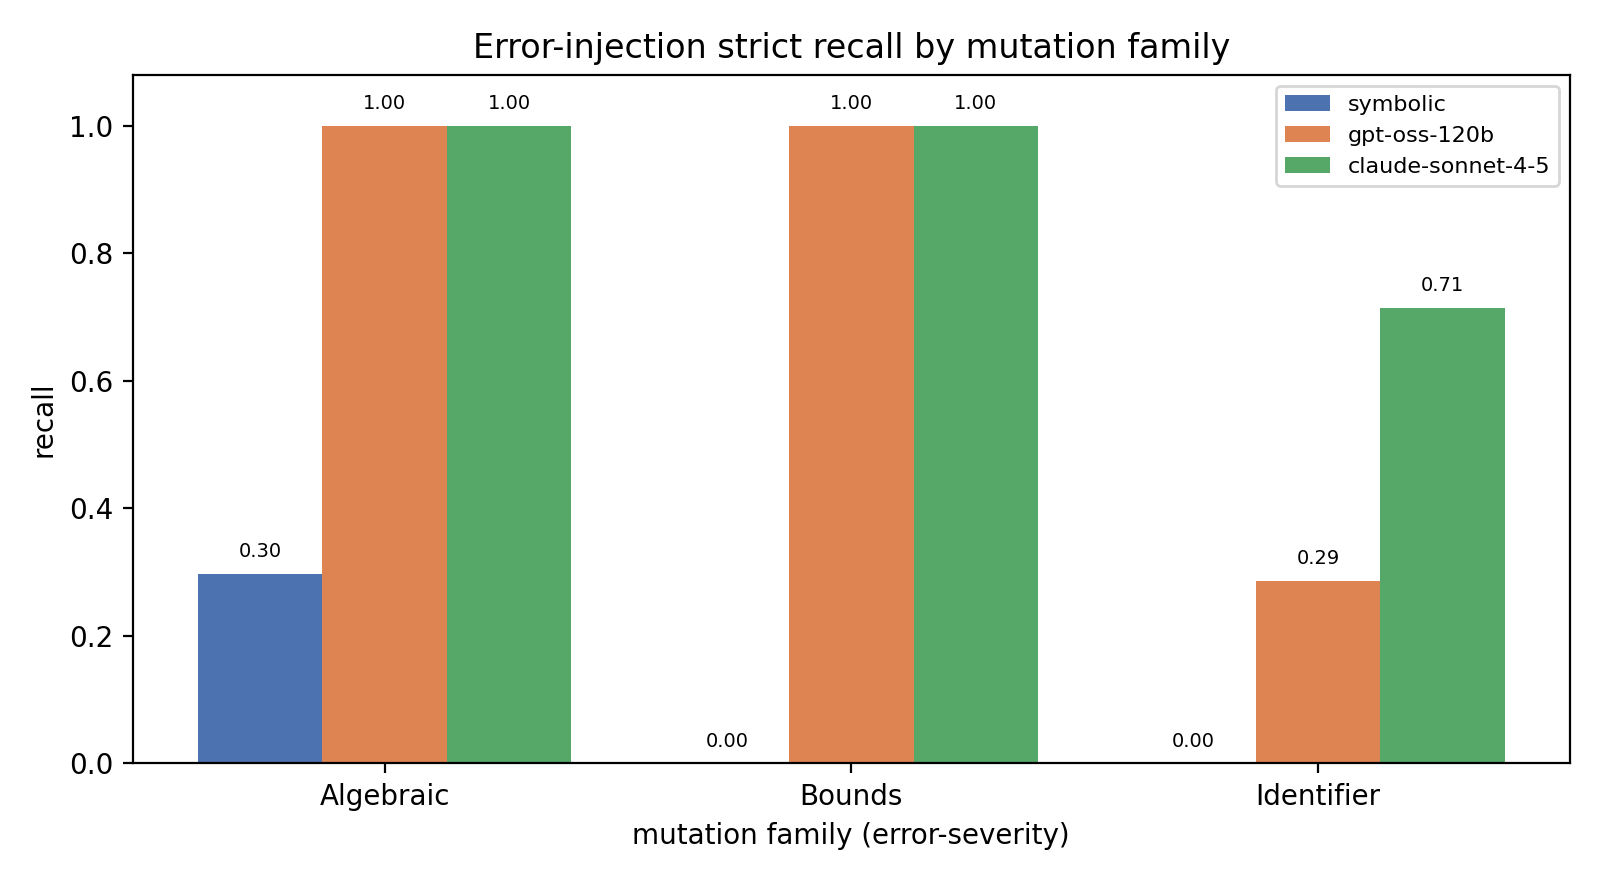
\includegraphics[width=\columnwidth]{../results/figures/fig2_injection_by_family.png}
\caption{Per-family \emph{strict} recall on the injection suite (error-severity
families only: $n{=}74$ algebraic, $6$ bounds, $14$ identifier graded trials).
Symbolic recall is $0.00$ on bounds and identifier (full abstention); nonzero
detection is confined to algebraic mutations. LLM judges cover all families.}
\label{fig:fig2}
\end{figure}
